%%%%%%%%%%%%%%%%%%%%%%%%%%%%%%%%%%%%%%%%%%%%%%%%%%%
%% LaTeX book template                           %%
%% Author:  Swayam Jena %%
%% License: ISC license                          %%
%%%%%%%%%%%%%%%%%%%%%%%%%%%%%%%%%%%%%%%%%%%%%%%%%%%

\documentclass[a4paper,11pt]{book}
\usepackage[T1]{fontenc}
\usepackage[utf8]{inputenc}
\usepackage{lmodern}
%%%%%%%%%%%%%%%%%%%%%%%%%%%%%%%%%%%%%%%%%%%%%%%%%%%%%%%%%
% Source: http://en.wikibooks.org/wiki/LaTeX/Hyperlinks %
%%%%%%%%%%%%%%%%%%%%%%%%%%%%%%%%%%%%%%%%%%%%%%%%%%%%%%%%%
\usepackage[dvipsnames]{xcolor}
\definecolor{RED}{named}{red}

\usepackage{hyperref}
\usepackage{graphicx}
\usepackage[english]{babel}
\usepackage{makecell}

%%%%%%%%%%%%%%%%%%%%%%%%%%%%%%%%%%%%%%%%%%%%%%%%%%%%%%%%%%%%%%%%%%%%%%%%%%%%%%%%
% 'dedication' environment: To add a dedication paragraph at the start of book %
% Source: http://www.tug.org/pipermail/texhax/2010-June/015184.html            %
%%%%%%%%%%%%%%%%%%%%%%%%%%%%%%%%%%%%%%%%%%%%%%%%%%%%%%%%%%%%%%%%%%%%%%%%%%%%%%%%
\newenvironment{dedication}
{
   \cleardoublepage
   \thispagestyle{empty}
   \vspace*{\stretch{1}}
   \hfill\begin{minipage}[t]{0.66\textwidth}
   \raggedright
}
{
   \end{minipage}
   \vspace*{\stretch{3}}
   \clearpage
}

%%%%%%%%%%%%%%%%%%%%%%%%%%%%%%%%%%%%%%%%%%%%%%%%
% Chapter quote at the start of chapter        %
% Source: http://tex.stackexchange.com/a/53380 %
%%%%%%%%%%%%%%%%%%%%%%%%%%%%%%%%%%%%%%%%%%%%%%%%
\makeatletter
\renewcommand{\@chapapp}{}% Not necessary...
\newenvironment{chapquote}[2][2em]
  {\setlength{\@tempdima}{#1}%
   \def\chapquote@author{#2}%
   \parshape 1 \@tempdima \dimexpr\textwidth-2\@tempdima\relax%
   \itshape}
  {\par\normalfont\hfill--\ \chapquote@author\hspace*{\@tempdima}\par\bigskip}
\makeatother

%%%%%%%%%%%%%%%%%%%%%%%%%%%%%%%%%%%%%%%%%%%%%%%%%%%
% First page of book which contains 'stuff' like: %
%  - Book title, subtitle                         %
%  - Book author name                             %
%%%%%%%%%%%%%%%%%%%%%%%%%%%%%%%%%%%%%%%%%%%%%%%%%%%

% Book's title and subtitle
\title{\Huge \textbf{Science}  \footnote{This is a $5^{th}$ class  science book.} \\ \huge Sample book subtitle \footnote{This is book is taught at KT Global School.}}
% Author
\author{\textsc{First-name Last-name}\thanks{\url{www.swayamjena.com}}}


\begin{document}

\frontmatter
\maketitle

%%%%%%%%%%%%%%%%%%%%%%%%%%%%%%%%%%%%%%%%%%%%%%%%%%%%%%%%%%%%%%%
% Add a dedication paragraph to dedicate your book to someone %
%%%%%%%%%%%%%%%%%%%%%%%%%%%%%%%%%%%%%%%%%%%%%%%%%%%%%%%%%%%%%%%
\begin{dedication}
Dedicated to Baba.
\end{dedication}

%%%%%%%%%%%%%%%%%%%%%%%%%%%%%%%%%%%%%%%%%%%%%%%%%%%%%%%%%%%%%%%%%%%%%%%%
% Auto-generated table of contents, list of figures and list of tables %
%%%%%%%%%%%%%%%%%%%%%%%%%%%%%%%%%%%%%%%%%%%%%%%%%%%%%%%%%%%%%%%%%%%%%%%%
\tableofcontents
\listoffigures
\listoftables

\mainmatter

%%%%%%%%%%%
% Preface %
%%%%%%%%%%%
\chapter*{Preface}
to be filled

\section*{Un-numbered sample section}
to be filled

\section*{Another sample section}
to be filled

\section*{Structure of book}
% You might want to add short description about each chapter in this book.
Each unit will focus on <SOMETHING>.

\section*{About the companion website}
The website\footnote{\url{https://github.com/swayam-jena/ScienceBook}} for this file contains:
\begin{itemize}
  \item A link to (freely downlodable) latest version of this document.
  \item Link to download LaTeX source for this document.
  \item Miscellaneous material (e.g. suggested readings etc).
\end{itemize}

%%%%%%%%%%%%%%%%%%%%%%%%%%%%%%%%%%%%
% Give credit where credit is due. %
% Say thanks!                      %
%%%%%%%%%%%%%%%%%%%%%%%%%%%%%%%%%%%%
\section*{Acknowledgements}
\begin{itemize}
\item A special word of thanks goes to Professor Knuth\footnote{\url{http://www-cs-faculty.stanford.edu/~uno/}} (for \TeX{}) and Leslie Lamport\footnote{\url{http://www.lamport.org/}} (for \LaTeX{}).
\item I'll also like to thank Gummi\footnote{\url{http://gummi.midnightcoding.org/}} developers and LaTeXila\footnote{\url{http://projects.gnome.org/latexila/}} development team for their awesome \LaTeX{} editors.
\item I'm deeply indebted my parents, colleagues and friends for their support and encouragement.
\end{itemize}
\mbox{}\\
%\mbox{}\\
\noindent Swayam Jena \\
\noindent \url{http://www.swayamjena.com}

%%%%%%%%%%%%%%%%
% NEW CHAPTER! %
%%%%%%%%%%%%%%%%
\chapter{Dignity of Labour}

\begin{chapquote}{Unknown author, \textit{Unknown source of this quote}}
'Every occupation is important. Each occupation requires different skills and experience.'
\end{chapquote}

\section{Get Rolling}
Name the occupation of people you see in images given below and answer the questions that follow\\
\begin{enumerate}
    \item Which of the above occupations would like to choose when you grow up and what factors would influence your choice?\\
    \item Which occupations would you not choose? Give reasons for your answer.
\end{enumerate}
\section{Learning objectives}
\begin{itemize}
    \item to discuss that people do different types of work
    \item to classify workers into different types
    \item to recognize the importance of everyone's work and the dignity of labour
    \item to analyze the reasons responsible for child labour    
\end{itemize}

%%%%%%%%%%%%%%%%
% NEW CHAPTER! %
%%%%%%%%%%%%%%%%
\chapter{Food and Health}
\begin{chapquote}{Unknown author, \textit{Unknown source of this quote}}
'Role of nutrients, roughage and water in keeping healthy, communicable and non-communicable diseases, and prevention are treatment of diseases.'
\end{chapquote}

\section{Get rolling}
Look at Riya and her freinds. can you tell who has healthy habits? Write Good for healthy habits and Bad for unhealthy ones in the spaces provided.
\begin{itemize}
    \item Riya loves to exercise everyday. \textcolor{green}{Good}
    \item Rohan loves to eat burger and fried food daily. \textcolor{red}{Bad}
    \item Sirman always uses handkerchief while sneezing. \textcolor{green}{Good}
    \item Sia always forgets to cover her mouth while coughing. \textcolor{red}{Bad}
    \item Ruhi loves to eat salad. \textcolor{green}{Good}
\end{itemize}
\section{Learning Objectives}
\begin{itemize}
    \item to recall the role of nutrients in the body
    \item to explain a food pryamid
    \item to discuss different deficiency diseases 
    \item to differentiate between communicable and non-comminucable diseases
\end{itemize}
\section{\textcolor{red}{Nutrients in food}}
We eat food to live and stay healthy. Food provides us with energy and helps in the growth, development and repair of the body. Food also protects us from various diseases. All these functions of food are possible due to the presence of \textcolor{red}{nutrients} in it.\\
\par
There are different types of nutrients, and they all have different 
roles. Let us have a quick recap of nutrients and their roles.
\subsection{\textcolor{orange}{Types of nutrients}}
Nutrients from food, including carbohydrates in items like bread and rice, fat from  sources like nuts and olive oil, are vital for energy and organ protection. Protiens found in dairy products, fish and meat help in growth and body repair. Vitamins and minerals, obtained from fruits and vegetables, support overall health.
\subsection{\textcolor{orange}{Roughage and Water}}
In addition to the essential nutrients, we also require sufficient roughage and water in our diet. Roughage, derived from whole grains and fruits, aids digestion and prevents \textcolor{red}{constipation}. Water is important for temperature regulation, digestion, and transportation of nutrients in the body. Drinking enough water helps us stay hydrated, which is essential for the proper functioning of the body.

\begin{figure}[h]
    \centering
    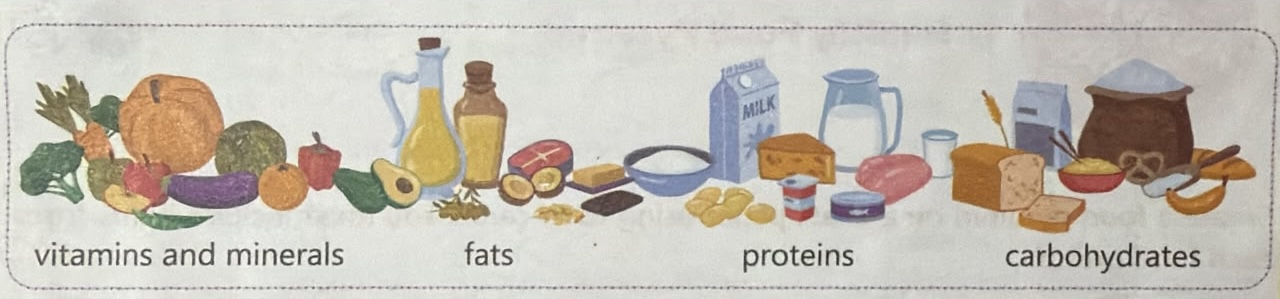
\includegraphics[scale=0.28]{image/food.jpeg}
    \caption{Nutritious Food}
    \label{fig:placeholder}
\end{figure}
\section{\textcolor{red}{Food Pyramid}}
Dietary requirements vary from person to person. Every person has unique factors that influence his or her nutritional needs of a person are age, gender, activity level are health condition. \\
\par

A \textbf{food pyramid} is a visual representation of a balanced diet, showing the different food groups are their recommended quantities for healthy and balanced nutrition.\\
\par
A typical food pyramid consists of several horizontal sections of layers, with each layer representing a different food group.

\begin{figure}[h]
    \centering
    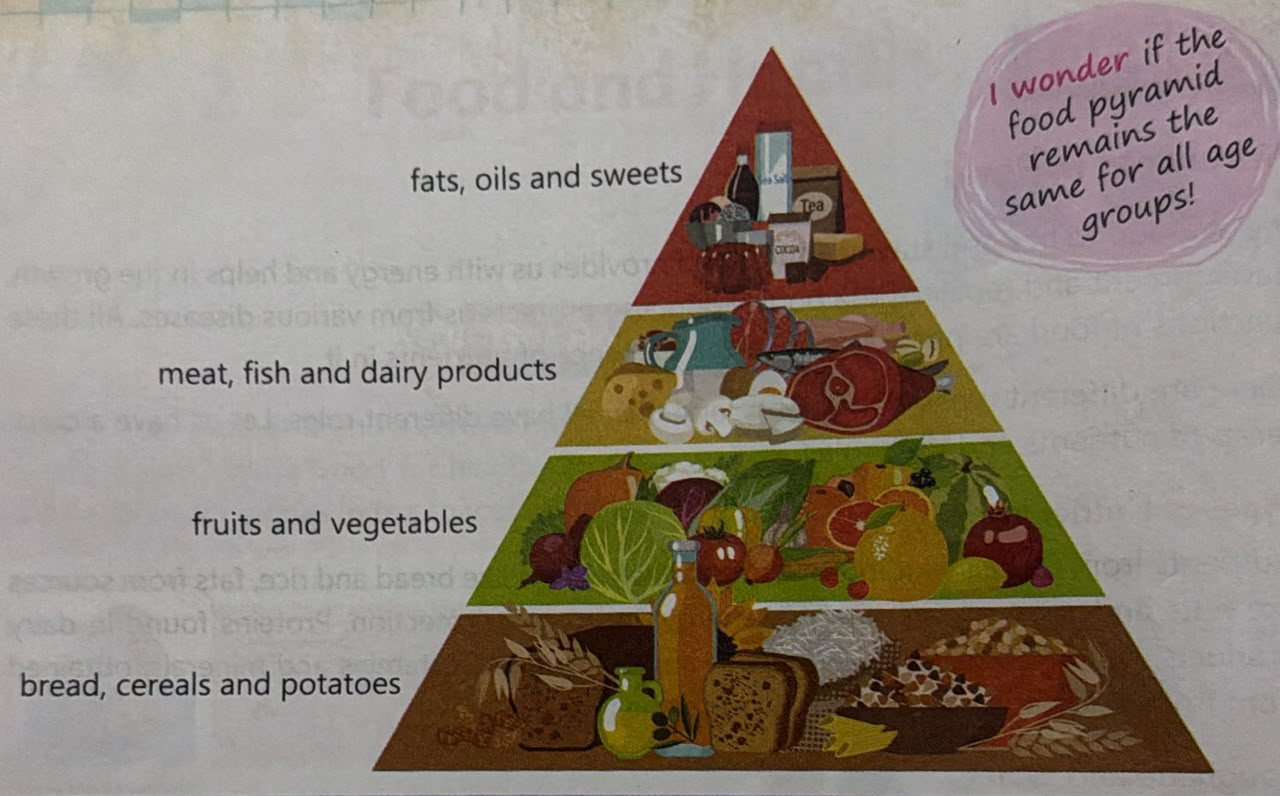
\includegraphics[scale=0.28]{image/food-pyramid.jpeg}
    \caption{ Food Pyramid}
    \label{fig:placeholder}
\end{figure}

Not eating balanced diet or eating a diet that is deficient in one or more nutrients leads to a deficiency of those nutrients in the body. Such a deficiency  of nutrients may lead to \textbf{deficiency diseases.}\\
\par
Let us first understand what diseases are.\\

\section{\textcolor{red}{Diseases}}
When we fall sick, we do not feel like doing anything. This condition when the body is unable to function properly is called a disease. \\
\par
Diseases can be of two types, \textbf{communicable} and \textbf{non-comminucable} depending on whether they can spread one person to another or not.
\section{\textcolor{red}{Non-Communicable Diseases}}
The diseases that do not spread from one person to another are called \textbf{non-communicable diseases.} All deficiency diseases are non-communicable diseases. Let us learn about deficiency diseases.\\ 
\subsection{\textcolor{orange}{Deficiency diseases}}
\textbf{Deficiency diseases} are caused by lack of one more nutrients in the diet. Some common deficiency diseases are their \textcolor{red}{symptom} are summarised in th table below.\\

  \pagebreak
\begin{table}[!h]
    \centering  
\begin{tabular}{|c|c|p{3.7cm}|p{3.4cm}|}
\hline
 \makecell{\textbf{Deficiency} \\ \textbf{disease}} & \makecell{\textbf{Deficiency} \\ \textbf{cause}} & \makecell{\textbf{Common symptoms}} & \makecell{  \textbf{Food to be eaten} \\ \textbf{to avoid deficiency}} \\
 \hline
 anaemia & iron & fatigue, weakness and \textcolor{red}{pale} skin & red meat, poultry, fish, beans, lentils, tofu and spinach\\
 \hline
goitre & iodine & englargement of a gland in the neck region & iodised salt and seafood\\
\hline
tooth decay & calcium & weak and teeth bones & milk, milk products, sprouts, multi-grain cereals and sesame seeds\\
\hline
\makecell{night \\blindness} & vitamin A & poor vision at night & carrots, sweet potatoes, pumpkin, spinach and cod liver oil\\
\hline 
beriberi & vitamin B & extreme tiredness, loss of appetite and loss of muscle function & fish, chicken, eggs, kidney beans and daily products\\
\hline
scurvy & vitamin C & bleeding gums, swelling of joints and impaired wound healing & oranges, lemons, grapefruits, strawberries, kiwi and tomatoes\\
\hline
rickets & vitamin D & weak and brittle bones & egg yolk, milk, mushroom and cod liver oil\\
\hline
marasmus & carbohydrates, proteins, and fats & serve weight loss, fatigue and weakness, and growth impairment and dry and loose skin & rice, wheat, bread, pulses, eggs, milk and fish\\
\hline
kwashiorkor & proteins & scaly skin, thin legs, swollen stomach and ankles & pulses, milk, fish and eggs\\
\hline
\end{tabular}
\caption{Deficiency disease, there cause and food to prevent them}
\end{table}

\section{\textcolor{red}{Overnutrition}}
\textbf{Overnutrition}, or excessive nutrient intake, occurs when a person consumes more nutrients than needed, leading to \textbf{obesity.} Obesity is characterised by excess fat deposits in one's body. If often results from the overconsumption of carbohydrates and fats that are not adequately utilised by the body. This can lead to health issues like high blood pressure and heart diseases.\\
\par
Excessive consumption of junk food, which how is low in nutritional value and high in carbohydrates, sugars, unhealthy fats and salt, in major cause obesity. Examples of junk food include burgers, pizzas, candies, cookies, cakes, pastries, soda, noodles, energy drinks and sweetened juices.
\section{\textcolor{red}{Communicable Diseases}}
\textbf{Communicable diseases} are illensses that can pass from one person to another. These diseases are caused by tiny organisms called \textbf{germs,} which are generally microbes. Microbes are too small to be seen without a microscope. Common types of microbes include bacteria, viruses, protozoa and funji.
\subsection{\textcolor{orange}{Direct Contact}}
Some germs can be transferred through direct physical contact with an infected person. Diseases such as common cold, chickenpox and mealseas spread in this way.
\begin{figure}[h]
    \centering
    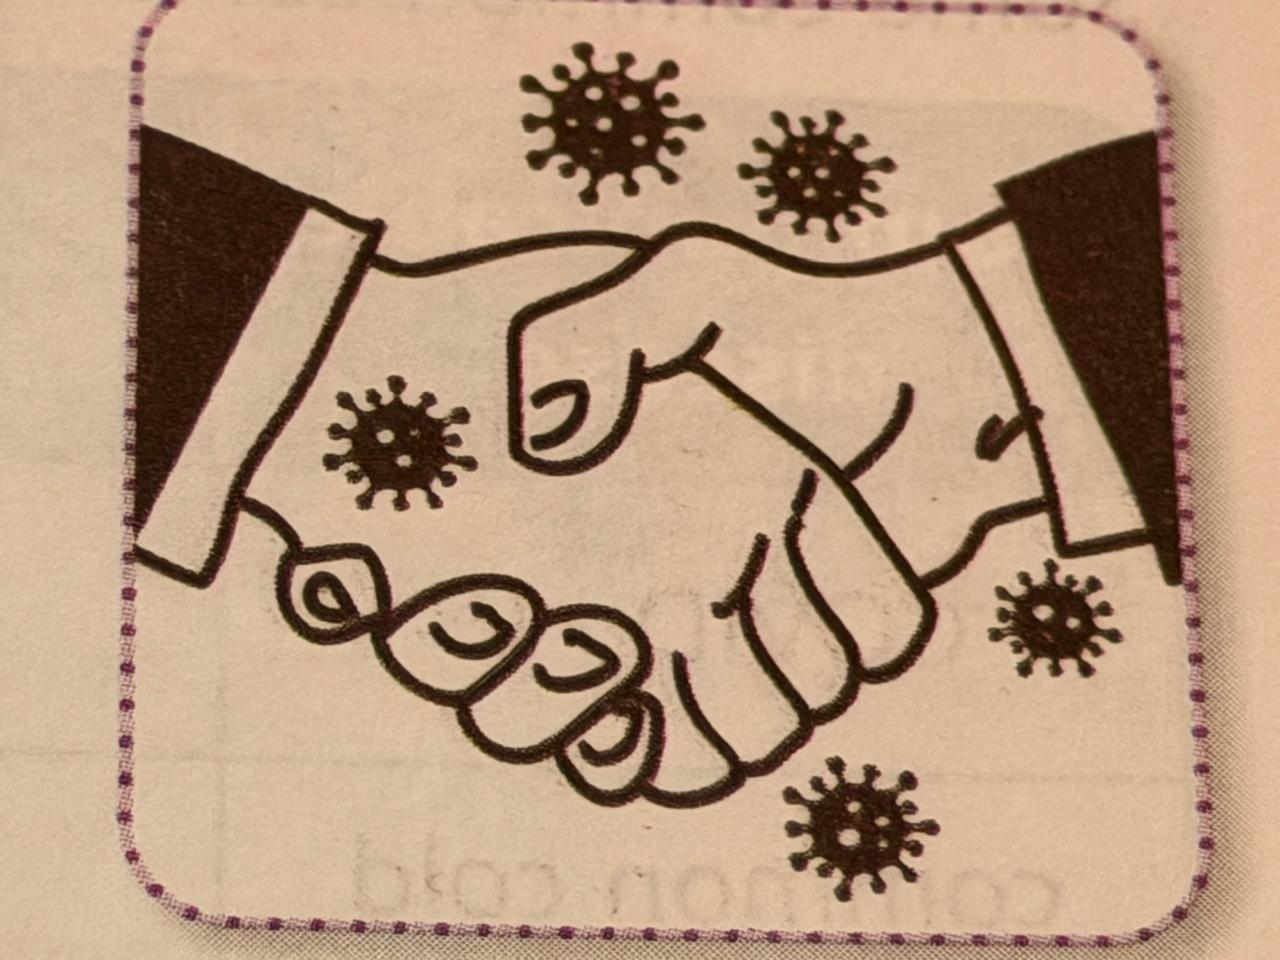
\includegraphics[width=0.5\linewidth]{image/contact.jpeg}
    \caption{Transfer of disease through handshake}
    \label{fig:placeholder}
\end{figure}
\subsection{\textcolor{orange}{Indirect Contact}} 
Germs can also be transferred indirectly through objects or surfaces; for example, by touching a doorknob or a surface that has been touched by an infected person and then touching the face. COVID-19 can spread in this manner.
\begin{figure}
    \centering
    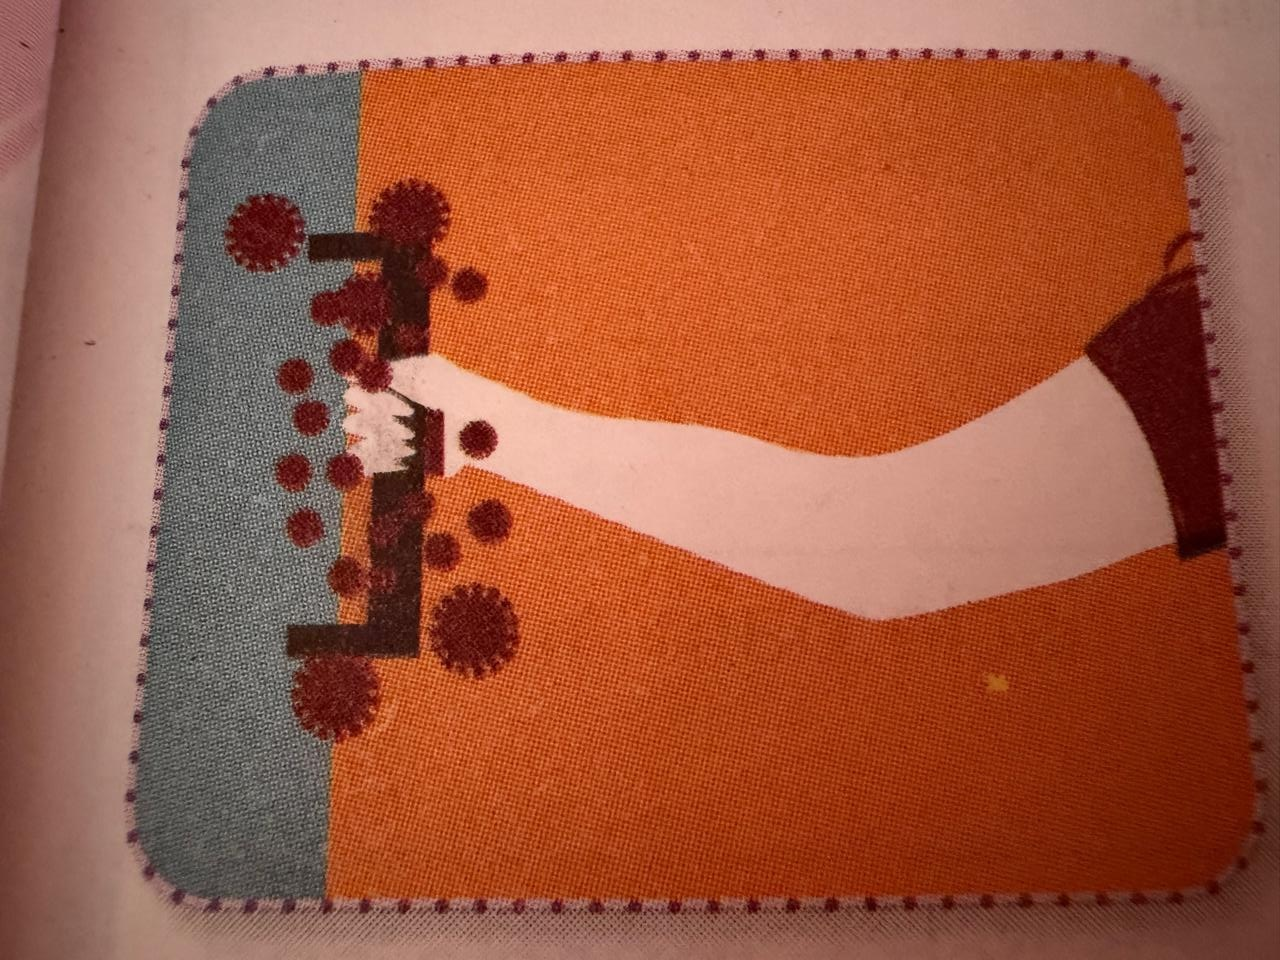
\includegraphics[width=0.5\linewidth]{image/hand.jpeg}
    \caption{Diseases through Indirect Contact}
    \label{fig:placeholder}
\end{figure}
\subsection{\textcolor{orange}{Through Air}}
Certain diseases spread when germs are realeased into the air through coughing, sneezing or talking by an infected person. People nearby can inhale these germs, making them infected. Example of such diseases include common cold and whooping cough.
\begin{figure}[!h]
    \centering
    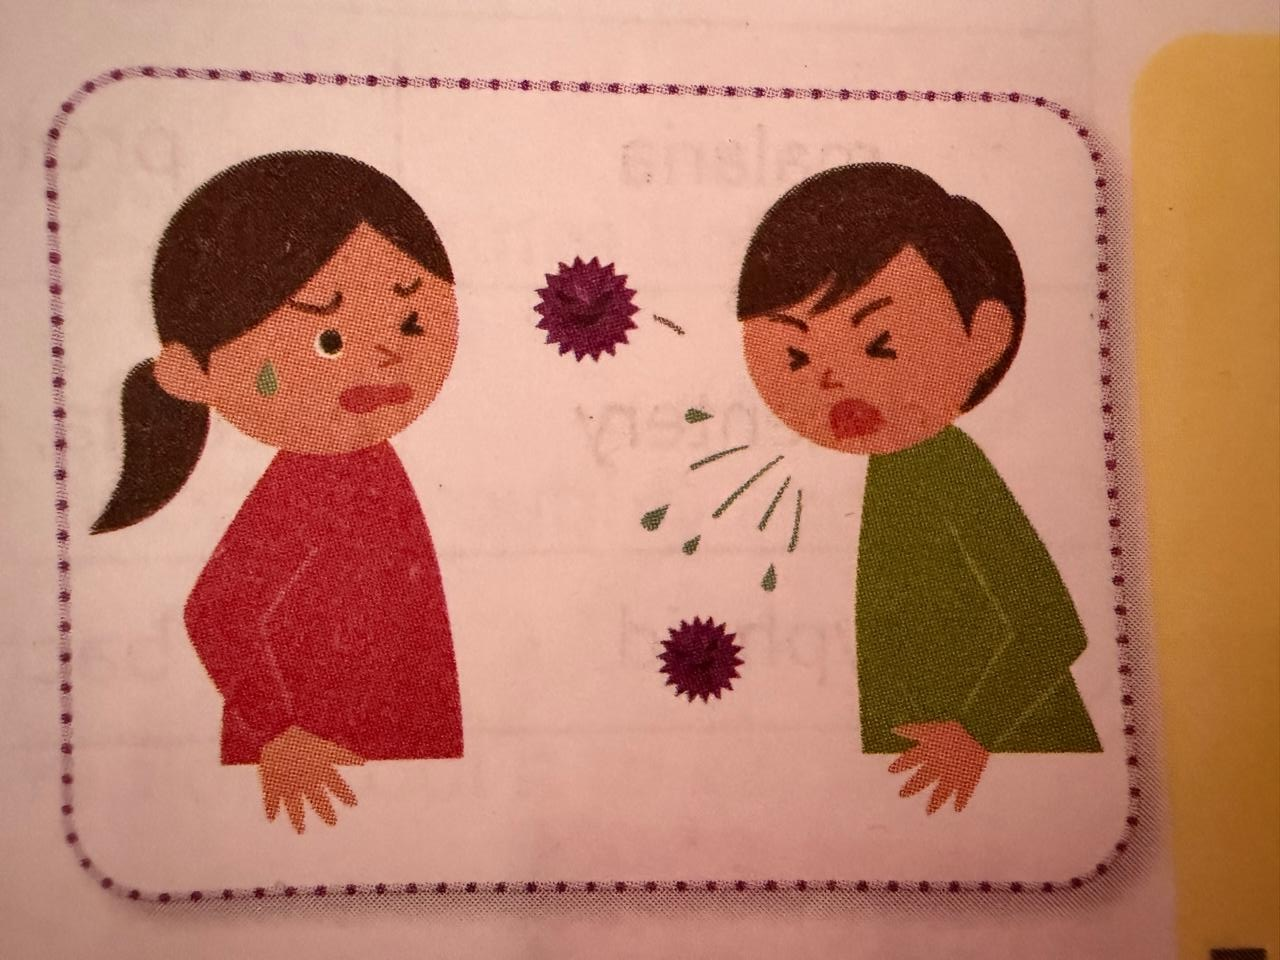
\includegraphics[width=0.5\linewidth]{image/air.jpeg}
    \caption{Caption}
    \label{fig:placeholder}
\end{figure}

\subsection{\textcolor{orange}{Through Water}}
\textcolor{red}{Contaminated} water sources carry germs that cause diseases like cholera and dysentery. When people consume or come into contact with contaminated water, they become infected and acquire such diseases.
\subsection{\textcolor{orange}{Through Food}}
Consuming contaminated food or beverages can lead to the transfer of certain germs, resulting in diseases like diarrhoea and jaundice.

\begin{figure}[!h]
    \centering
    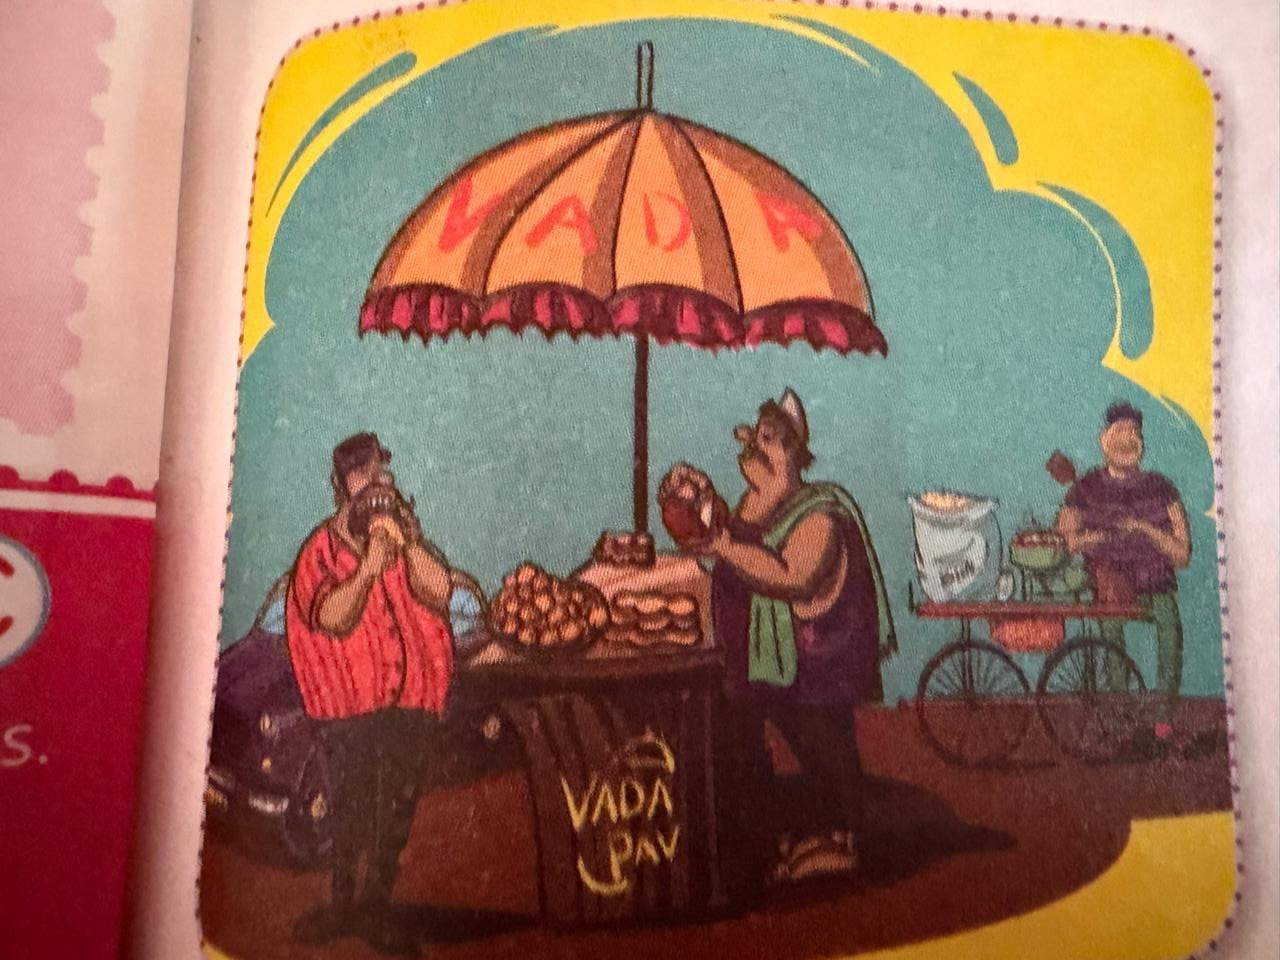
\includegraphics[width=0.5\linewidth]{image/contaminated_food.jpeg}
    \caption{Contaminated Through Food}
    \label{fig:placeholder}
\end{figure}

\subsection{\textcolor{orange}{Through Flies and Mosquitoes}}
Certain diseases are transferred by flies and mosquitoes. Flies sit on food, contaminate it and act as a carrier of germs. Mosquitoes suck blood of a person infected with malaria and then bite someone, causing that person to become infected. This way, mosquitoes too act as a carrier of germs.

\begin{figure}[!h]
    \centering
    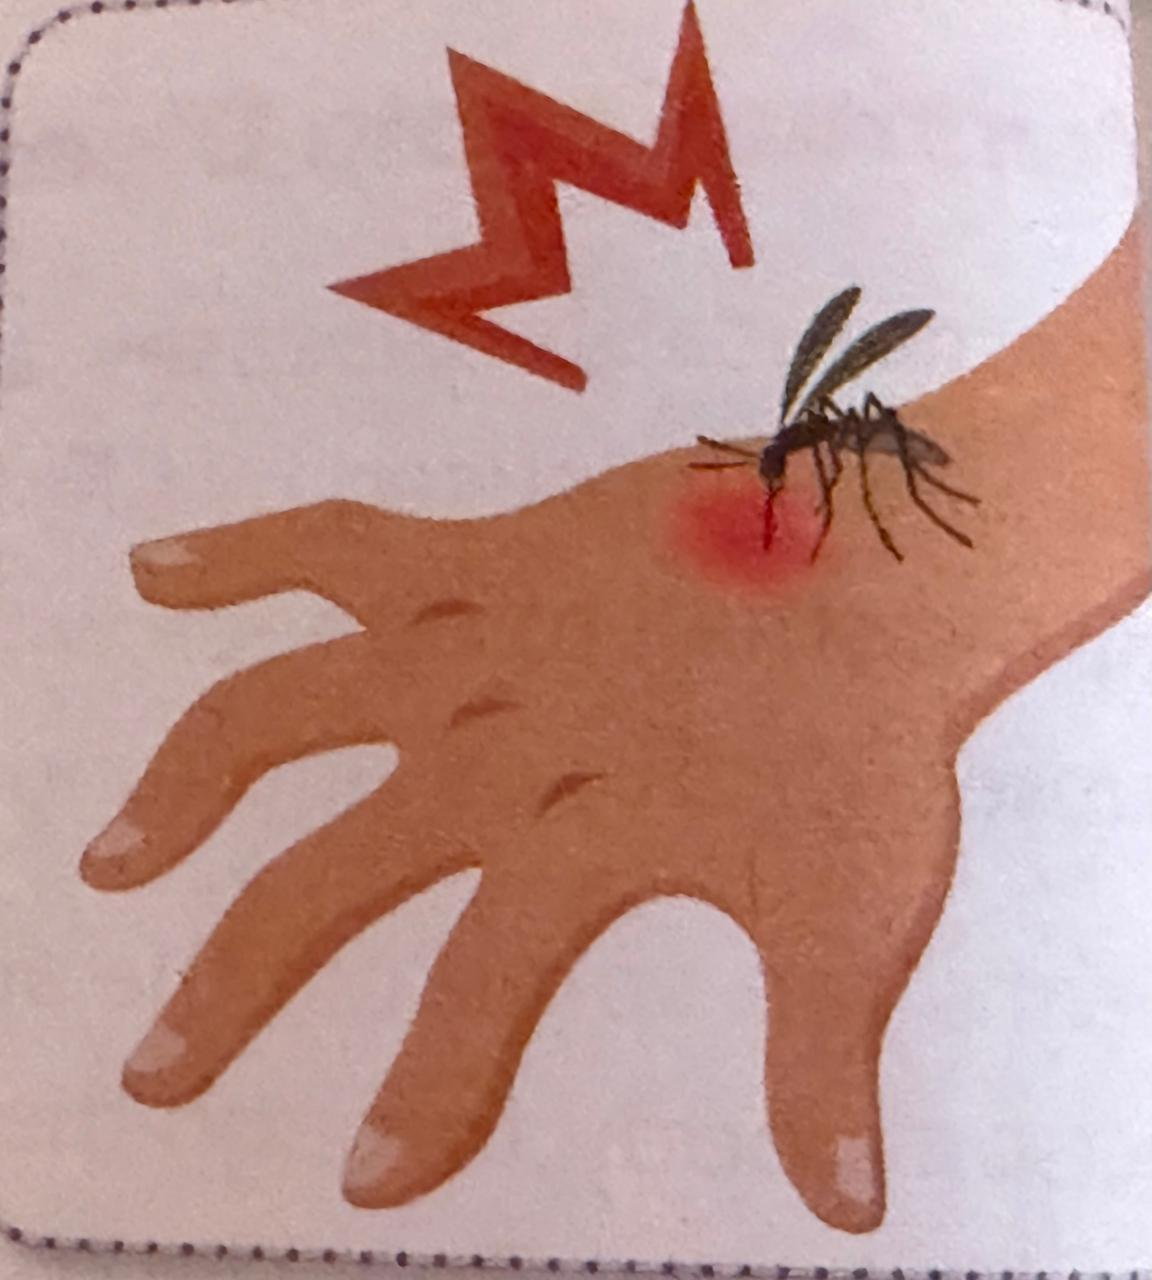
\includegraphics[width=0.5\linewidth]{image/mosquito_bite.jpeg}
    \caption{Diseases through flies and mosquitoes}
    \label{fig:placeholder}
\end{figure}

Some common communicable diseases are summarised in the table below.
\begin{table}[!h]
\centering
    
    \begin{tabular}{|c|c|c|}
    \hline
\textbf{Communicable diseases} & \textbf{Cause} & \textbf{Symptoms} \\
\hline
COVID-19 & virus & cough, cold, fever, sore throat and shortness of breath\\
\hline
common cold & virus & cough, cold and sore throat\\
\hline
measles & virus & runny nose, sore throat, white sports inside the mouth and fever\\
\hline
chickenpox & virus & rashes, fever and body pain\\
\hline
dengue & virus & high fever, rashes, joint and muscle pain and tiredness\\
\hline
malaria & protozoa & fever, chills, headache, stomach ache, muscle and joint pain\\
\hline
dysentery & bacteria, protozoa & diarrhoea, stomach ache, fever, dehydration, and vomiting\\
\hline
typhoid & bacteria & fever, tierdness, loss of appetite and stomach ache\\
\hline
    \end{tabular}
    \caption{Caption}
    \label{tab:placeholder}
\end{table}




\end{document}
